\documentclass{beamer}
\usepackage{tikz}
\usepackage{xcolor}

\definecolor{darkgreen}{rgb}{0.0, 0.7, 0.13}
\setbeamertemplate{navigation symbols}{}%remove navigation symbols

\begin{document}

\begin{frame}
%\frametitle{Non-identifiability of rate and times}

\begin{columns}
\column{0.4\textwidth}
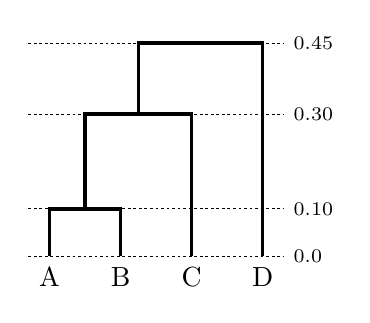
\begin{tikzpicture}[yscale=-0.55,xscale=0.55]
  \draw[dash pattern=on 1.0 off 1.0 ] (-14pt, 140pt) -- (154pt, 140pt);
  \node[anchor=west, dash pattern=on 1.0 off 1.0 ] at (154pt, 140pt) {\scriptsize{0.0}};
  \draw[dash pattern=on 1.0 off 1.0 ] (-14pt, 108.88889pt) -- (154pt, 108.88889pt);
  \node[anchor=west, dash pattern=on 1.0 off 1.0 ] at (154pt, 108.88889pt) {\scriptsize{0.10}};
  \draw[dash pattern=on 1.0 off 1.0 ] (-14pt, 46.66667pt) -- (154pt, 46.66667pt);
  \node[anchor=west, dash pattern=on 1.0 off 1.0 ] at (154pt, 46.66667pt) {\scriptsize{0.30}};
  \draw[dash pattern=on 1.0 off 1.0 ] (-14pt, 0pt) -- (154pt, 0pt);
  \node[anchor=west, dash pattern=on 1.0 off 1.0 ] at (154pt, 0pt) {\scriptsize{0.45}};
  \node[anchor=north, line width=1.25pt] at (0pt, 140pt) {A};
  \node[anchor=north, line width=1.25pt] at (46.66667pt, 140pt) {B};
  \draw[line width=1.25pt] (0pt, 140pt) -- (0pt, 108.88889pt) -- (23.33333pt, 108.88889pt);
  \draw[line width=1.25pt] (46.66667pt, 140pt) -- (46.66667pt, 108.88889pt) -- (23.33333pt, 108.88889pt);
  \node[anchor=north, line width=1.25pt] at (93.33334pt, 140pt) {C};
  \draw[line width=1.25pt] (23.33333pt, 108.88889pt) -- (23.33333pt, 46.66667pt) -- (58.33333pt, 46.66667pt);
  \draw[line width=1.25pt] (93.33333pt, 140pt) -- (93.33333pt, 46.66667pt) -- (58.33333pt, 46.66667pt);
  \node[anchor=north, line width=1.25pt] at (140pt, 140pt) {D};
  \draw[line width=1.25pt] (58.33333pt, 46.66667pt) -- (58.33333pt, 0pt) -- (99.16667pt, 0pt);
  \draw[line width=1.25pt] (140pt, 140pt) -- (140pt, 0pt) -- (99.16667pt, 0pt);
\end{tikzpicture}
\column{0.2\textwidth}

\centering
$=\quad\textcolor{darkgreen}{0.01}\quad\times$

\column{0.4\textwidth}
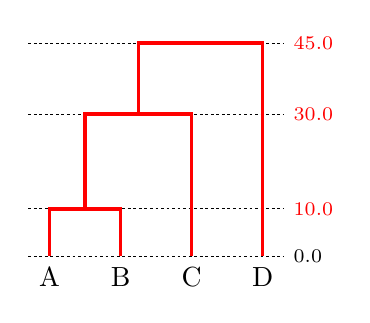
\begin{tikzpicture}[yscale=-0.55,xscale=0.55]
  \draw[dash pattern=on 1.0 off 1.0 ] (-14pt, 140pt) -- (154pt, 140pt);
  \node[anchor=west, dash pattern=on 1.0 off 1.0 ] at (154pt, 140pt) {\scriptsize{0.0}};
  \draw[dash pattern=on 1.0 off 1.0 ] (-14pt, 108.88889pt) -- (154pt, 108.88889pt);
  \node[red,anchor=west, dash pattern=on 1.0 off 1.0 ] at (154pt, 108.88889pt) {\scriptsize{10.0}};
  \draw[dash pattern=on 1.0 off 1.0 ] (-14pt, 46.66667pt) -- (154pt, 46.66667pt);
  \node[red,anchor=west, dash pattern=on 1.0 off 1.0 ] at (154pt, 46.66667pt) {\scriptsize{30.0}};
  \draw[dash pattern=on 1.0 off 1.0 ] (-14pt, 0pt) -- (154pt, 0pt);
  \node[red,anchor=west, dash pattern=on 1.0 off 1.0 ] at (154pt, 0pt) {\scriptsize{45.0}};
  \node[anchor=north, line width=1.25pt] at (0pt, 140pt) {A};
  \node[anchor=north, line width=1.25pt] at (46.66667pt, 140pt) {B};
  \draw[line width=1.25pt,red] (0pt, 140pt) -- (0pt, 108.88889pt) -- (23.33333pt, 108.88889pt);
  \draw[line width=1.25pt,red] (46.66667pt, 140pt) -- (46.66667pt, 108.88889pt) -- (23.33333pt, 108.88889pt);
  \node[anchor=north, line width=1.25pt] at (93.33334pt, 140pt) {C};
  \draw[line width=1.25pt,red] (23.33333pt, 108.88889pt) -- (23.33333pt, 46.66667pt) -- (58.33333pt, 46.66667pt);
  \draw[line width=1.25pt,red] (93.33333pt, 140pt) -- (93.33333pt, 46.66667pt) -- (58.33333pt, 46.66667pt);
  \node[anchor=north, line width=1.25pt] at (140pt, 140pt) {D};
  \draw[line width=1.25pt,red] (58.33333pt, 46.66667pt) -- (58.33333pt, 0pt) -- (99.16667pt, 0pt);
  \draw[line width=1.25pt,red] (140pt, 140pt) -- (140pt, 0pt) -- (99.16667pt, 0pt);
\end{tikzpicture}

\end{columns}

\begin{columns}
\column{0.4\textwidth}
\column{0.2\textwidth}

\centering
$=\quad\textcolor{darkgreen}{\mathbf{0.1}}\quad\times$

\column{0.4\textwidth}
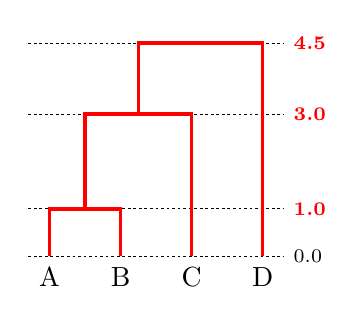
\begin{tikzpicture}[yscale=-0.55,xscale=0.55]
  \draw[dash pattern=on 1.0 off 1.0 ] (-14pt, 140pt) -- (154pt, 140pt);
  \node[anchor=west, dash pattern=on 1.0 off 1.0 ] at (154pt, 140pt) {\scriptsize{0.0}};
  \draw[dash pattern=on 1.0 off 1.0 ] (-14pt, 108.88889pt) -- (154pt, 108.88889pt);
  \node[red,anchor=west, dash pattern=on 1.0 off 1.0 ] at (154pt, 108.88889pt) {\scriptsize{\bf1.0}};
  \draw[dash pattern=on 1.0 off 1.0 ] (-14pt, 46.66667pt) -- (154pt, 46.66667pt);
  \node[red,anchor=west, dash pattern=on 1.0 off 1.0 ] at (154pt, 46.66667pt) {\scriptsize{\bf3.0}};
  \draw[dash pattern=on 1.0 off 1.0 ] (-14pt, 0pt) -- (154pt, 0pt);
  \node[red,anchor=west, dash pattern=on 1.0 off 1.0 ] at (154pt, 0pt) {\scriptsize{\bf4.5}};
  \node[anchor=north, line width=1.25pt] at (0pt, 140pt) {A};
  \node[anchor=north, line width=1.25pt] at (46.66667pt, 140pt) {B};
  \draw[line width=1.25pt,red] (0pt, 140pt) -- (0pt, 108.88889pt) -- (23.33333pt, 108.88889pt);
  \draw[line width=1.25pt,red] (46.66667pt, 140pt) -- (46.66667pt, 108.88889pt) -- (23.33333pt, 108.88889pt);
  \node[anchor=north, line width=1.25pt] at (93.33334pt, 140pt) {C};
  \draw[line width=1.25pt,red] (23.33333pt, 108.88889pt) -- (23.33333pt, 46.66667pt) -- (58.33333pt, 46.66667pt);
  \draw[line width=1.25pt,red] (93.33333pt, 140pt) -- (93.33333pt, 46.66667pt) -- (58.33333pt, 46.66667pt);
  \node[anchor=north, line width=1.25pt] at (140pt, 140pt) {D};
  \draw[line width=1.25pt,red] (58.33333pt, 46.66667pt) -- (58.33333pt, 0pt) -- (99.16667pt, 0pt);
  \draw[line width=1.25pt,red] (140pt, 140pt) -- (140pt, 0pt) -- (99.16667pt, 0pt);
\end{tikzpicture}

\end{columns}

\medskip{}

\begin{columns}
\column{0.33\textwidth}
\centering
``substitution tree''
\column{0.33\textwidth}
\centering
evolutionary rate
\scriptsize{substitutions / site / unit time}
\column{0.33\textwidth}
\centering
time tree
\end{columns}
\end{frame}
\end{document}
